\chapter{Они назвали его Lisp неспроста: обработка списков}
\label{ch:12}

Списки в языке Lisp играют важную роль как по историческим, так и по практическим
причинам. Изначально списки были основным составным типом данных в языке Lisp, и в течение
десятилетий они были \textit{единственным} составным типом данных. В наши дни программист на
Common Lisp может использовать как типы vector, hash table, самостоятельно определённые
типы и структуры, так и списки.

Списки остаются в языке потому, что они являются прекрасным решением для определённого
рода проблем. Одна из них~-- проблема представления кода как данных для трансформации и
генерации кода в макросах~-- является специфичной для языка Lisp, и это объясняет то, как
другие языки обходятся без списков в стиле Lisp. Вообще говоря, списки~-- прекрасная
структура данных для представления любых неоднородных и/или иерархических данных. Кроме
того, они достаточно легковесны и поддерживают функциональный стиль программирования~-- ещё
одна важная часть наследия Lisp.

Итак, вы должны понять списки в их собственных терминах; после того как вы достигнете
хорошего понимания того, как списки работают, вы сможете лучше оценивать, стоит ли их
использовать или нет.

\section{Списков нет}

Мальчик с ложкой: Не пытайся согнуть список. Это невозможно. Вместо этого... попытайся
понять истину.

Нео: Какую истину?

Мальчик с ложкой: Списков нет.

Нео: Списков нет?

Мальчик с ложкой: И тогда ты поймёшь: это не списки, которые сгибаются; это только ты
сам\footnote{Перифраз из к/ф <<Матрица>>.
  \href{http://us.imdb.com/Quotes?0133093}{Оригинальная цитата}.}.

Ключом к пониманию списков является осознание того, что они, по большей части, иллюзия,
построенная на основе объектов более примитивных типов данных. Эти простые объекты~-- пары
значений, называемые \textit{cons-ячейками} (\textit{cons cells}), от имени функции
\lstinline{CONS}, используемой для их создания.

\lstinline{CONS} принимает 2 аргумента и возвращает новую cons-ячейку, содержащую 2 значения
\footnote{\lstinline{CONS}~-- сокращения для глагола construct~-- конструировать.}. Эти значения
могут быть ссылками на объект любого типа. Если второе значение не \lstinline{NIL} и не другая
cons-ячейка, то ячейка печатается как два значения в скобках, разделённые точкой (так
называемая точечная пара).

\begin{myverb}
(cons 1 2) ==> (1 . 2)
\end{myverb}

Два значения в cons-ячейке называются \lstinline{CAR} и \lstinline{CDR}~-- по имени функций,
используемых для доступа к ним. На заре времён эти имена были мнемониками, по крайней мере
для людей, работающих над первой реализацией Lisp на IBM 704. Но даже тогда они были всего
лишь позаимствованы из мнемоник ассемблера, используемых для реализации этих операций. Тем
не менее это не так уж плохо, что названия данных функций несколько бессмысленны,
применительно к конкретной cons-ячейке лучше думать о них просто как о произвольной паре
значений без какого-либо особого смысла. Итак:

\begin{myverb}
(car (cons 1 2)) ==> 1
(cdr (cons 1 2)) ==> 2
\end{myverb}

Оба \lstinline{CAR} и \lstinline{CDR} могут меняться функцией \lstinline{SETF}: если дана cons-ячейка, то
можно присвоить значение обеим её составляющим\footnote{Когда место, переданное в
  \lstinline{SETF},~-- это \lstinline{CAR} или \lstinline{CDR}, вызов \lstinline{SETF} разворачивается в вызов
  функции \lstinline{RPLACA} или \lstinline{RPLACD}; некоторые лисперы старой школы, те самые, что
  до сих пор используют \lstinline{SETQ}, будут применять \lstinline{RPLACA} или \lstinline{RPLACD}
  непосредственно, но современный стиль учит использовать \lstinline{SETF} для \lstinline{CAR} и
  \lstinline{CDR}.}.

\begin{myverb}
(defparameter *cons* (cons 1 2))
*cons*                 ==> (1 . 2)
(setf (car *cons*) 10) ==> 10
*cons*                 ==> (10 . 2)
(setf (cdr *cons*) 20) ==> 20
*cons*                 ==> (10 . 20)
\end{myverb}

Так как значения в cons-ячейке могут быть ссылками на любой объект, вы можете строить большие
структуры, связывая cons-ячейки между собой. Списки строятся связыванием cons-ячеек в
цепочку. Элементы списка содержатся в \lstinline{CAR} cons-ячеек, а связи со следующими
cons-ячейками содержатся в их \lstinline{CDR}. Последняя ячейка в цепочке имеет \lstinline{CDR} со
значением \lstinline{NIL}, которое, как я говорил в главе~\ref{ch:04}, представляет собой как
пустой список, так и булево значение ложь.

Такая компоновка отнюдь не уникальна для Lisp, она называется \textit{односвязный
список} (\textit{singly linked list}). Несколько языков, не входящих в семейство Lisp,
предоставляют расширенную поддержку для этого скромного типа данных.

Таким образом, когда я говорю, что какое-то значение является списком, я имею в виду, что
оно либо \lstinline{NIL}, либо ссылка на cons-ячейку. \lstinline{CAR} cons-ячейки является первым
элементом списка, а \lstinline{CDR} является ссылкой на другой список (который, в свою очередь,
также является cons-ячейкой), содержащий остальные элементы или значение
\lstinline{NIL}. Устройство вывода Lisp понимает это соглашение и печатает такие цепочки
cons-ячеек как списки в скобках, нежели как точечные пары.

\begin{myverb}
(cons 1 nil)                   ==> (1)
(cons 1 (cons 2 nil))          ==> (1 2)
(cons 1 (cons 2 (cons 3 nil))) ==> (1 2 3)
\end{myverb}

Когда мы говорим о структурах из cons-ячеек, нам могут помочь несколько диаграмм. Эти
диаграммы изображают cons-ячейки как пары блоков:

\begin{figure}[h]
  \centering
  
\includegraphics[scale=0.6]{images/one-cons-cell.png}
\end{figure}

Блок слева представляет \lstinline{CAR}, а блок справа~-- \lstinline{CDR}. Значения, хранимые в
ячейках, также представлены в виде отдельных блоков или в виде стрелки, выходящей из блока,
для представления ссылки на значение\footnote{Как правило, простые объекты, такие как
  числа, изображаются внутри соответствующего блока, а более сложные объекты~-- снаружи, со
  стрелкой, выходящей из блока, означающей ссылку. Это хорошо согласуется с тем, как
  работают многие реализации Common Lisp: хотя все объекты концептуально хранятся как
  ссылки, некоторые простые неизменяемые объекты могут храниться в cons-ячейках
  непосредственно.}. Например, список \lstinline{(1 2 3)}, который состоит из трёх cons-ячеек,
связанных вместе с помощью их \lstinline{CDR}, может быть изображён так:

\begin{figure}[h]
  \centering
  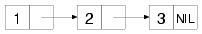
\includegraphics[scale=0.6]{images/list-1-2-3.png}
\end{figure}

Однако в основном при работе со списками вы не обязаны иметь дело с отдельными ячейками,
поскольку существуют функции, которые создают списки и используются для манипулирования
ими. Например, функция \lstinline{LIST} строит cons-ячейки и связывает их вместе, следующие
\lstinline{LISP}-выражения эквивалентны \lstinline{CONS}-выражениям, приведённым выше:

\begin{myverb}
(list 1)     ==> (1)
(list 1 2)   ==> (1 2)
(list 1 2 3) ==> (1 2 3)
\end{myverb}

Аналогично, когда вы думаете в терминах списков, вы не должны использовать бессмысленные
имена \lstinline{CAR} и \lstinline{CDR}; вы должны использовать \lstinline{FIRST} и \lstinline{REST}~--
синонимы для \lstinline{CAR} и \lstinline{CDR} при рассмотрении cons-ячеек как списков.

\begin{myverb}
(defparameter *list* (list 1 2 3 4))
(first *list*)        ==> 1
(rest *list*)         ==> (2 3 4)
(first (rest *list*)) ==> 2
\end{myverb}

Как и cons-ячейки, списки могут содержать значения любых типов.

\begin{myverb}
(list "foo" (list 1 2) 10) ==> ("foo" (1 2) 10)
\end{myverb}

Структура списка при этом выглядит так:

\begin{figure}[h]
  \centering
  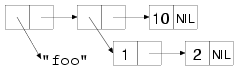
\includegraphics[scale=0.6]{images/mixed-list.png}
\end{figure}

Поскольку элементами списка могут быть другие списки, то с помощью списков можно представлять
деревья произвольной глубины и сложности. Таким образом, они идеально подходят для
представления гетерогенных иерархических данных. Например, XML-процессоры, основанные на
Lisp, как правило, представляют XML-документы в виде списков. Другим очевидным примером
данных с древовидной структурой является сам код на языке Lisp. В главах~\ref{ch:30} и
\ref{ch:31} вы
напишете библиотеку для генерации HTML-кода, которая использует списки списков для
представления кода, который необходимо сгенерировать. В следующей главе я расскажу больше
об использовании cons-ячеек для представления других типов данных.

Common Lisp предоставляет обширную библиотеку функций для работы со списками. В
разделах~\ref{sec:12-list-funcs} и~\ref{sec:12-map} вы узнаете о наиболее важных из
них. Данные функции будет проще понять в контексте идей, взятых из парадигмы
функционального программирования.

\section{Функциональное программирование и списки}

Суть функционального программирования~-- в том, что программы состоят исключительно из
функций без побочных эффектов, которые вычисляют свои значения исключительно на основе
своих аргументов. Преимущество функционального стиля программирования~-- в том, что он
облегчает понимание программы. Устранение побочных эффектов ведёт к устранению практически
всех возможностей удалённого воздействия. Так как результат функции определяется её
аргументами, поведение функции легче понять и протестировать. Например, когда вы видите
выражение \lstinline{(+ 3 4)}, вы знаете, что результат целиком задаётся определением функции
\lstinline{+} и переданными аргументами 3 и 4. Вам не надо беспокоиться о том, что могло
произойти в программе до этого, так как нет ничего, что могло бы изменить результат
вычисления выражения.

Функции, работающие с числами, естественным образом являются функциональными, так как числа
неизменяемы. Списки же, как вы видели раннее, могут меняться при применении функции
\lstinline{SETF} над ячейками списка. Тем не менее списки могут рассматриваться как
функциональные типы данных, если считать, что их значение определяется элементами, которые
они содержат. Так, любой список вида \lstinline{(1 2 3 4)} функционально эквивалентен любому
другому списку, содержащему эти четыре значения, независимо от того, какие cons-ячейки
используются для представления списка. И любая функция, которая принимает списки в
качестве аргументов и возвращает значение, основываясь исключительно на содержании списка,
могут считаться функциональными. Например, если функции \lstinline{REVERSE} передать список
\lstinline{(1 2 3 4)}, она всегда вернёт \lstinline{(4 3 2 1)}. Различные вызовы \lstinline{REVERSE} с
функционально-эквивалентными аргументами вернут функционально-эквивалентные
результаты. Другой аспект функционального программирования, который я рассматриваю в
разделе~\ref{sec:12-map},~-- это использование функций высших порядков: функций, которые
используют другие функции как данные, принимая их в качестве аргументов или возвращая в
качестве результата.

Большинство функций Common Lisp для работы со списками написано в функциональном
стиле. Позднее мы обсудим, как совмещать функциональный подход к программированию с другими
подходами, но сначала вы должны понять некоторые тонкости функционального подхода
применительно к спискам.

Так как большинство функций для работы со списками написано в функциональном стиле, они могут
возвращать результаты, которые имеют общие cons-ячейки с их аргументами. Возьмём
конкретный пример: функция \lstinline{APPEND} принимает любое число списков в качестве
аргументов и возвращает новый список, содержащий все элементы списков-аргументов,
например:

\begin{myverb}
(append (list 1 2) (list 3 4)) ==> (1 2 3 4)
\end{myverb}

С точки зрения функционального подхода, задача функции \lstinline{APPEND}~-- вернуть список
\lstinline{(1 2 3 4)}, не изменяя ни одну из cons-ячеек в списках-аргументах \lstinline{(1 2)} и
\lstinline{(3 4)}. Очевидно, что это можно сделать создав, новый список, состоящий из четырёх
новых cons-ячеек. Однако в этом есть лишняя работа. Вместо этого \lstinline{APPEND} на самом
деле создаёт только две новые cons-ячейки, чтобы хранить значения 1 и 2, соединяя их
вместе и делая ссылку из \lstinline{CDR} второй ячейки на первый элемент последнего аргумента~--
списка \lstinline{(3 4)}. После этого функция возвращает cons-ячейку, содержащую 1. Ни одна из
входных cons-ячеек не была изменена, и результатом, как и требовалось, является список
\lstinline{(1 2 3 4)}. Единственная хитрость в том, что результат, возвращаемый функцией
\lstinline{APPEND}, имеет общие cons-ячейки со списком \lstinline{(3 4)}. Структура результата
выглядит так:

\begin{figure}[h]
  \centering
  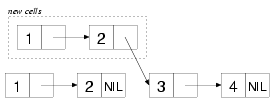
\includegraphics[scale=0.6]{images/after-append.png}
\end{figure}

В общем случае функция \lstinline{APPEND} должна копировать все, кроме последнего,
аргументы-списки, и она может вернуть результат, который \textit{имеет общие данные} с
последним аргументом.

Другие функции также используют полезную особенность списков иметь общие
структуры. Некоторые, как и \lstinline{APPEND}, всегда возвращают результаты, которые имеют
общие структуры со своими аргументами. Другим функциям позволено возвращать результаты с
общими структурами, но это зависит от их реализации.

\section{<<Разрушающие>> операции}

Если бы Common Lisp был строго функциональным языком, больше не о чем было бы
говорить. Однако, так как после создания cons-ячейки есть возможность изменить её значение,
применив функцию \lstinline{SETF} над её \lstinline{CAR} и \lstinline{CDR}, мы должны обсудить, как
стыкуются побочные эффекты и общие структуры.

Из-за функционального наследия языка Lisp операции, которые изменяют существующие объекты,
называются \textit{разрушающими} (\textit{destructive})~-- в функциональном программировании
изменение состояния объекта <<разрушает>> его, так как объект больше не представляет того же
значения, что до применения функции. Однако использование одного и того же термина для
обозначения всего класса операций, изменяющих состояние существующих объектов, ведёт к некоторой
путанице, так как существует два сильно отличающихся класса таких операций:
операции \textit{для побочных эффектов} (\textit{for-side-effect} operations) и
\textit{утилизирующие} операции (\textit{recycling} operations)\footnote{Термин <<\textit{для
  побочных эффектов}>> используется в стандарте языка, термин же <<\textit{утилизирующие}>>~--
  моё изобретение; большинство пособий по Lisp использует термин <<\textit{разрушающие}>> для
  обоих классов, я же пытаюсь развеять неразбериху.}.

Операции для побочных эффектов~-- это те, которые используются ради их эффектов. В этом
смысле всякое использование \lstinline{SETF} является разрушающим, как и использование
функций, которые вызывают \lstinline{SETF}, чтобы изменить состояние объектов, например
\lstinline{VECTOR-PUSH} или \lstinline{VECTOR-POP}. Но это несколько некорректно~-- объявлять операции
разрушающими, так как они не предназначены для написания программ в функциональном стиле,
то есть они не могут быть описаны с использованием терминов функциональной парадигмы. Тем не
менее если вы смешиваете нефункциональные операции для побочных эффектов с функциями,
возвращающими результаты с общими структурами, то надо быть внимательным, чтобы случайно
не изменить эти общие структуры. Например, имеем:

\begin{myverb}
(defparameter *list-1* (list 1 2))
(defparameter *list-2* (list 3 4))
(defparameter *list-3* (append *list-1* *list-2*))
\end{myverb}

После вычисления у вас три списка, но \lstinline{list-3} и \lstinline{list-2} имеют общую
структуру, как показано на предыдущей диаграмме.

\begin{myverb}
*list-1*                  ==> (1 2)
*list-2*                  ==> (3 4)
*list-3*                  ==> (1 2 3 4)
\end{myverb}

Посмотрим, что случится, если мы изменим \lstinline{list-2}:

\begin{myverb}
(setf (first *list-2*) 0) ==> 0
*list-2*                  ==> (0 4)     ; как и ожидалось
*list-3*                  ==> (1 2 0 4) ; а вот этого возможно вы и не хотели
\end{myverb}

Из-за наличия общих структур изменения в списке \lstinline{list-2} привели к изменению списка
\lstinline{list-3}: первая cons-ячейка в \lstinline{list-2} является также третьей ячейкой в
\lstinline{list-3}. Изменение значения \lstinline{FIRST} списка \lstinline{list-2} изменило значение
\lstinline{CAR} в cons-ячейке, изменив оба списка.

Совсем по-другому обстоит дело с утилизирующими операциями, которые предназначены для
запуска в функциональном коде. Они используют побочные эффекты лишь для оптимизации. В
частности, они повторно используют некоторые cons-ячейки своих аргументов для получения
результатов. Но в отличие от таких функций, как \lstinline{APPEND}, которые используют
cons-ячейки, включая их без изменений в результирующий список, утилизирующие операции
используют cons-ячейки как сырьё, изменяя их \lstinline{CAR} и \lstinline{CDR} для получения
желаемого результата. Таким образом утилизирующие операции спокойно могут быть
использованы, когда их аргументы не пригодятся после их выполнения.

Чтобы понять, как работают функции утилизации, сравним неразрушающую операцию
\lstinline{REVERSE}, которая возвращает инвертированный аргумент, с функцией \lstinline{NREVERSE},
которая является утилизирующей функцией и делает то же самое. Так как \lstinline{REVERSE} не
меняет своих аргументов, она создаёт новую cons-ячейку для каждого элемента
списка-аргумента. Но предположим, вы напишите:

\begin{myverb}
(setf *list* (reverse *list*))
\end{myverb}

Присвоив результат вычисления переменной \lstinline{*list*}, вы удалили ссылку на начальное
значение \lstinline{*list*}. Если на cons-ячейки в начальном списке больше никто не ссылается,
то они теперь доступны для сборки мусора. Тем не менее в большинстве реализаций Lisp более
эффективным является повторно использовать эти ячейки, чем создавать новые, а старые
превращать в мусор.

\lstinline{NREVERSE} именно это и делает. \lstinline{N}~-- от <<\textit{несоздающая}>> (\textit{non-consing}),
в том смысле, что она не создаёт новых cons-ячеек. Конкретные побочные эффекты \lstinline{NREVERSE}
явно не описываются, она может проводить любые модификации над \lstinline{CAR} и \lstinline{CDR}
любых cons-ячеек аргумента, но типичная реализация может быть такой: проход по списку с
изменением \lstinline{CDR} каждой cons-ячейки так, чтобы она указывала на предыдущую
cons-ячейку, в конечном счёте результатом будет cons-ячейка, которая была последней в
списке-аргументе, а теперь является головой этого списка. Никакие новые cons-ячейки при
этом не создаются, и сборка мусора не производится.

Большинство утилизирующих функций, таких как \lstinline{NREVERSE}, имеют своих неразрушающих
двойников, которые вычисляют тот же результат. В общем случае утилизирующие функции имеют
такое же имя, как их неразрушающие двойники с подставленной первой буквой N. Но есть и
исключения, например часто используемые: \lstinline{NCONC}~-- утилизирующая версия
\lstinline{APPEND} и \lstinline{DELETE}, \lstinline{DELETE-IF}, \lstinline{DELETE-IF-NOT},
\lstinline{DELETE-DUPLICATED}~-- версии семейства функций \lstinline{REMOVE}.

В общем случае вы можете использовать утилизирующие функции таким же образом, как их
неразрушающие аналоги, учитывая, что они безопасны, если их аргументы не будут
использованы после выполнения функций. Побочные эффекты большинства утилизирующих функций
недостаточно строго описаны, чтобы на них можно было полагаться.

Однако ещё большую неразбериху вносит небольшой набор утилизирующих функций со строго
определёнными побочными эффектами, на которые можно положиться. В этот набор входят
\lstinline{NCONC}, утилизирующая версия \lstinline{APPEND} и \lstinline{NSUBSTITUTE}, а также её \lstinline{-IF} и
\lstinline{-IF-NOT} варианты~-- утилизирующие версии группы функций \lstinline{SUBSTITUTE}.

Как и \lstinline{APPEND}, \lstinline{NCONC} возвращает соединение своих аргументов, но строит такой
результат следующим образом: для каждого непустого аргумента-списка \lstinline{NCONC}
устанавливает в \lstinline{CDR} его последней cons-ячейки ссылку на первую cons-ячейку
следующего непустого аргумента-списка. После этого она возвращает первый список, который
теперь является головой результата-соединения. Таким образом:

\begin{myverb}
(defparameter *x* (list 1 2 3))
(nconc *x* (list 4 5 6)) ==> (1 2 3 4 5 6)
*x*                      ==> (1 2 3 4 5 6)
\end{myverb}

На функцию \lstinline{NSUBSTITUTE} и её варианты можно положиться в следующем её поведении: она
пробегает по списковой структуре аргумента-списка и устанавливает с помощью функции
\lstinline{SETF} новое значения в \lstinline{CAR} его cons-ячеек. После этого она возвращает
переданный ей аргумент-список, который теперь имеет то же значение, как если бы был
вычислен с помощью \lstinline{SUBSTITUTE}\footnote{Строковые функции
  \lstinline{NSTRING-CAPITALIZE}, \lstinline{NSTRING-DOWNCASE}, и \lstinline{NSTRING-UPCASE} действуют
  так же: они возвращают такой же результат, как их аналоги без \lstinline{N}, но при этом
  изменяют свои аргументы.}.

Ключевой момент, который необходимо запомнить о \lstinline{NCONC} и \lstinline{NSUBSTITUTE}, состоит
в том, что они являются исключением из правила не полагаться на побочные эффекты
утилизирующих функций. Вполне допустимо, и даже желательно, игнорировать возможность
полагаться на побочные эффекты этих функций и использовать их, как и любые другие
утилизирующие функции, только ради возвращаемых ими значений.

\section{Комбинирование утилизации с общими структурами}

Хотя вы можете спокойно использовать утилизирующие функции, если их аргументы не будут
использованы позднее, стоит заметить, что каждая утилизирующая функция~-- как заряженное
ружье, направленное на собственную ногу, в том смысле, что если вы случайно примените
утилизирующую функцию к аргументу, который используете позднее, то наверняка потеряете
пару пальцев.

Всё усложняется тем, что функции, использующие общие структуры, и утилизирующие функции
работают над схожими задачами. Неразрушающие списочные функции возвращают списки,
которые имеют общие структуры со своими аргументами, основываясь на предположении, что
cons-ячейки этих общих структур никогда не поменяются, а утилизирующие функции работают с
нарушением этого допущения. Другими словами, использование общих структур основано на
предположении, что вам безразлично, какие cons-ячейки составляют результат, утилизирующие
же функции требуют, чтобы вы точно знали, откуда берутся cons-ячейки.

На практике утилизирующие функции используются в нескольких определённых
случаях. Наиболее частый случай~-- построение списка, который будет возвращён из функции
добавлением элементов в его конец (как правило, с использованием функции \lstinline{PUSH}), а
потом инвертирование данного списка. При этом список хранится в локальной для данной
функции переменной\footnote{При анализе кода из Common Lisp Open Code Collection
  (CLOCC), выясняется, что среди множества библиотек, написанных разными авторами,
  сочетание \lstinline{PUSH} и \lstinline{NREVERSE} составляет около половины всех использований
  утилизирующих функций.}.

Это является эффективным способом построения списка, потому что каждый вызов \lstinline{PUSH}
создаёт только одну cons-ячейку, а вызов \lstinline{NREVERSE} быстро пробегает по списку,
переназначая \lstinline{CDR} ячеек. Так как список создаётся в локальной переменной внутри
функции, то не существует никакой возможности того, что какой-то код за пределами функции имеет общие
структуры с данным списком. Вот пример функции, использующей такой приём для
построения списка, содержащего числа от 0 до n\footnote{Конечно же имеются и другие
  пути достижения такого результата. Например, макрос \lstinline{LOOP} делает это очень просто
  и похоже генерирует код, который даже эффективнее связки \lstinline{PUSH}/\lstinline{NREVERSE}.}:

\begin{myverb}
(defun upto (max)
  (let ((result nil))
    (dotimes (i max)
      (push i result))
    (nreverse result)))

(upto 10) ==> (0 1 2 3 4 5 6 7 8 9)
\end{myverb}

Другой часто встречающийся случай применения утилизирующих функций\footnote{Использование
  этого случая насчитывает около 30\% от всех случаев использования утилизирующий функций
  в CLOCC.}~-- немедленное переприсваивание значения, возвращаемого утилизирующей функцией,
переменной, содержащей потенциально утилизированное значение. Например, вы часто будете
видеть такие выражения с использованием функций \lstinline{DELETE} (утилизирующей версии
\lstinline{REMOVE}):

\begin{myverb}
(setf foo (delete nil foo))
\end{myverb}

Эта конструкция присваивает переменной \lstinline{foo} её старое значение с удалёнными
элементами, равными \lstinline{NIL}. Однако здесь утилизирующие функции должны применяться
осмотрительно: если \lstinline{foo} имеет общие структуры с другими списками, то использование
\lstinline{DELETE} вместо \lstinline{REMOVE} может разрушить структуры этих списков. Например,
возьмём два списка \lstinline{list-2} и \lstinline{list-3}, рассмотренных ранее, они разделяют свои
последние две cons-ячейки.

\begin{myverb}
*list-2* ==> (0 4)
*list-3* ==> (1 2 0 4)
\end{myverb}

Вы можете удалить \lstinline{4} из \lstinline{list-3} так:

\begin{myverb}
(setf *list-3* (delete 4 *list-3*)) ==> (1 2 0)
\end{myverb}

Но \lstinline{DELETE}, скорее всего, произведёт удаление тем, что установит \lstinline{CDR} третьей
ячейки списка в \lstinline{NIL}, отсоединив таким образом четвёртую ячейку от
списка. Так как третья ячейка в \lstinline{list-3} является также первой ячейкой в \lstinline{list-2},
этот код изменит еще и \lstinline{list-2}:

\begin{myverb}
*list-2* ==> (0)
\end{myverb}

Если вы используете \lstinline{REMOVE} вместо \lstinline{DELETE}, то результат будет построен с
помощью создания новых ячеек, не изменяя ячеек \lstinline{list-3}. В этом случае \lstinline{list-2}
не будет изменён.

Эти два случая использования вместе составляют около 80\% от общего числа случаев
использования утилизирующих функций. Другие случаи использования возможны, но требуют
внимательного отслеживания того, возвращают ли функции списки с общими структурами или нет.

В общем случае при работе со списками лучше писать код в функциональном стиле~-- ваши
функции должны полагаться на содержание их аргументов-списков и не должны менять
их. Следование этому правилу, разумеется, исключает использование разрушающих операций,
утилизирующих или нет~-- не имеет значения. После того как вы получите работающий код и
профилирование покажет, что вам нужна оптимизация, вы можете заменить неразрушающие
операции со списками на их утилизирующие варианты, но только при условии, что аргументы
данных функций не используются где-то ещё.

Важный момент, на который следует обратить внимание: функции сортировки списков
\lstinline{SORT}, \lstinline{STABLE-SORT} и \lstinline{MERGE} из главы~\ref{ch:11} также являются
утилизирующими функциями, когда они применяются к спискам\footnote{\lstinline{SORT} и
  \lstinline{STABLE-SORT} могут также применяться к векторам ради их побочных эффектов, но
  так как они возвращают отсортированный вектор, то вы должны использовать эти функции только
  ради возвращаемого ими значения из соображений единого подхода и логичности.}. Эти
функции не имеют неразрушающих аналогов, так что если вам необходимо отсортировать списки,
не разрушая их, вы должны передать в сортирующую функцию копию списка, сделанную с помощью
\lstinline{COPY-LIST}. В любом случае, вы должны сохранить результат функции, так как исходный
аргумент-список будет разрушен. Например:

\begin{myverb}
CL-USER> (defparameter *list* (list 4 3 2 1))
*LIST*
CL-USER> (sort *list* #'<)
(1 2 3 4)                      ; кажется то, что надо
CL-USER> *list*
(4)                            ; упс!
\end{myverb}


\section{Функции для работы со списками}
\label{sec:12-list-funcs}

Теперь вы готовы взглянуть на библиотеку функций для работы со списками, которую
предоставляет Common Lisp.

Вы уже видели базовые функции для извлечения элементов списка: \lstinline{FIRST} и
\lstinline{REST}. Хотя вы можете получить любой элемент списка, комбинируя вызовы \lstinline{REST}
(для продвижения по списку) и \lstinline{FIRST} (для выделения элемента), это может быть
утомительным занятием. Поэтому Lisp предоставляет функции от \lstinline{SECOND} до \lstinline{TENTH},
извлекающие соответствующие элементы списка. Более общая функция \lstinline{NTH} принимает два
аргумента: индекс и список и возвращает n-ый (начиная с нуля) элемент списка. Также
существует функция \lstinline{NTHCDR}, принимающая индекс и список и возвращающая результат
n-кратного применения \lstinline{REST} к списку. Таким образом, \lstinline{(nthcdr 0 ...)}  просто
возвращает исходный список, а \lstinline{(nthcdr 1 ...)}  эквивалентно вызову
\lstinline{REST}. Имейте в виду, что ни одна из этих функций не является более производительной,
по сравнению с эквивалентной комбинацией \lstinline{FIRST} и \lstinline{REST}, так как нет иного
способа получить n-ый элемент списка без n-кратного вызова \lstinline{CDR}\footnote{\lstinline{NTH}
  приблизительно эквивалентна функции \lstinline{ELT}, но работает только на списках. В
  противоположность \lstinline{ELT}, \lstinline{NTH} принимает индекс как первый аргумент. Другая
  разница между ними состоит в том, что \lstinline{ELT} сигнализирует об ошибке при попытке
  доступа к элементу в позиции, превышающей или равной длине списка, в то время как
  \lstinline{NTH} вернёт \lstinline{NIL}}.

28 составных \lstinline{CAR}-\lstinline{CDR} функций составляют ещё одно семейство, которое вы можете время
от времени использовать. Имя каждой функции получается подстановкой до 4 букв A или D
между C и R, каждая A представляет вызов \lstinline{CAR}, а каждая D~-- \lstinline{CDR}. Таким
образом:

\begin{myverb}
(caar list)   === (car (car list))
(cadr list)   === (car (cdr list))
(cadadr list) === (car (cdr (car (cdr list))))
\end{myverb}

Обратите внимание, что многие из этих функций имеют смысл только применительно к спискам,
содержащим другие списки. Например, \lstinline{CAAR} возвращает \lstinline{CAR} от \lstinline{CAR}
исходного списка, таким образом, этот список должен иметь своим первым элементом
список. Другими словами, эти функции для работы скорее с деревьями, нежели со списками:

\begin{myverb}
(caar (list 1 2 3))                  ==> ошибка
(caar (list (list 1 2) 3))           ==> 1
(cadr (list (list 1 2) (list 3 4)))  ==> (3 4)
(caadr (list (list 1 2) (list 3 4))) ==> 3
\end{myverb}

В настоящее время эти функции не используются так часто, как раньше. Даже упёртые
Lisp-хакеры старой закалки стремятся избегать этих длинных комбинаций. Однако они
присутствуют в старом Lisp-коде, поэтому необходимо представлять, как они
работают\footnote{В частности, они использовались для извлечения различных частей
  выражения, переданного в макрос до того, как был изобретён неструктурированный список
  параметров FIXME. Например, вы могли разложить выражение

\begin{myverb}
(when (> x 10) (print x))
\end{myverb}

таким образом:

\begin{myverb}
;; условие
(cadr '(when (> x 10) (print x))) ==> (> X 10)

;; тело как список
(cddr '(when (> x 10) (print x))) ==> ((PRINT X))
\end{myverb}
}.

Функции \lstinline{FIRST}-\lstinline{TENTH}, \lstinline{CAR}, \lstinline{CADR} и т. д. могут также быть
использованы как аргумент к \lstinline{SETF}, если вы пишите в нефункциональном стиле.

\begin{table}[tb]
\begin{tabular}{|c|p{110mm}|}
\hline
Функция& \multicolumn{1}{c|}{Описание}\\
\hline
\code{LAST}     &Возвращает последнюю cons-ячейку в списке. Если вызывается с целочисленным аргументом n, возвращает n ячеек\\
\code{BUTLAST}  &Возвращает копию списка без последней cons-ячейки. Если вызывается с целочисленным аргументом n, исключает последние n ячеек\\
\code{NBUTLAST} &Утилизирующая версия \code{BUTLAST}; может изменять переданный список-аргумент, не имеет строго заданных побочных эффектов\\
\code{LDIFF}    &Возвращает копию списка до заданной cons-ячейки\\
\code{TAILP}    &Возвращает \code{TRUE}, если переданный объект является cons-ячейкой, которая является частью списка\\
\code{LIST*}    &Строит список, содержащий все переданные аргументы, кроме последнего, после этого присваивает \code{CDR} последней cons-ячейки списка последнему аргументу. То есть смесь \code{LIST} и \code{APPEND}\\
\code{MAKE-LIST}&Строит список из n элементов. Начальные элементы списка \code{NIL} или значение, заданное аргументом \code{:initial-element}\\
\code{REVAPPEND}&Комбинация \code{REVERSE} и \code{APPEND}; инвертирует первый аргумент как \code{REVERSE} и добавляет второй аргумент. Не имеет строго заданных побочных эффектов\\
\code{NRECONC}  &Утилизирующая версия предыдущей функции; инвертирует первый аргумент, как это делает \code{NREVERSE}, и добавляет второй аргумент. Не имеет строгих побочных эффектов\\
\code{CONSP}    &Предикат для тестирования, является ли объект cons-ячейкой\\
\code{ATOM}     &Предикат для тестирования, является ли объект не cons-ячейкой\\
\code{LISTP}    &Предикат для тестирования, является объект cons-ячейкой или \code{NIL}\\
\code{NULL}     &Предикат для тестирования, является ли объект \code{NIL}. Функционально эквивалентен функции \code{NOT}, но стилистически лучше использовать \code{NULL} при тестировании, является ли список \code{NIL}, а \code{NOT} для проверки булева выражения \code{FALSE}\\
\hline
\end{tabular}
  \caption{Другие функции для работы со списками}
  \label{table:12-other}
\end{table}

\section{Отображение}
\label{sec:12-map}

Другой важный аспект функционального стиля программирования~-- это использование функций
высших порядков, то есть функций, которые принимают функции в качестве аргументов или
возвращают функции. Вы видели несколько примеров функций высших порядков, таких как
\lstinline{MAP}, в предыдущей главе. Хотя \lstinline{MAP} может использоваться как со списками, так
и с векторами (то есть с любым типом последовательностей), Common Lisp также предоставляет 6
функций отображения специально для списков. Разница между этими шестью функциями в том, как
они строят свой результат, и в том, применяют они переданные функции к элементам списка
или к cons-ячейкам списка.

\lstinline{MAPCAR}~-- функция, которая наиболее похожа на \lstinline{MAP}. Так как она всегда возвращает список,
она не требует уточнения типа результата, как \lstinline{MAP}. Вместо этого первый аргумент
\lstinline{MAPCAR}~-- функция, которую необходимо применить, а последующие аргументы~-- списки,
чьи элементы будут поставлять аргументы для этой функции. Другими словами, \lstinline{MAPCAR}
ведёт себя, как \lstinline{MAP}: функция применяется к элементам аргументов-списков, беря от
каждого списка по элементу. Результат каждого вызова функции собирается в новый
список. Например:

\begin{myverb}
(mapcar #'(lambda (x) (* 2 x)) (list 1 2 3)) ==> (2 4 6)
(mapcar #'+ (list 1 2 3) (list 10 20 30))    ==> (11 22 33)
\end{myverb}

\lstinline{MAPLIST} работает как \lstinline{MAPCAR}, только вместо того, чтобы передавать функции
элементы списка, она передаёт cons-ячейки\footnote{То есть \lstinline{MAPLIST} более примитивная
  из двух функций: если у вас есть только \lstinline{MAPLIST}, вы можете построить на её основе
  \lstinline{MAPCAR}, но построить \lstinline{MAPLIST} на основе \lstinline{MAPCAR} невозможно.}.  Таким
образом, функция имеет доступ не только к значению каждого элемента списка (через функцию
\lstinline{CAR}, применённую к cons-ячейке), но и к хвосту списка (через \lstinline{CDR}).

\lstinline{MAPCAN} и \lstinline{MAPCON} работают как \lstinline{MAPCAR} и \lstinline{MAPLIST}, разница состоит
в том, как они строят свой результат. В то время как \lstinline{MAPCAR} и \lstinline{MAPLIST} строят
новый список, содержащий результаты вызова функций, \lstinline{MAPCAN} и \lstinline{MAPCON} строят
результат склеиванием результатов (которые должны быть списками), как это делает
\lstinline{NCONC}. Таким образом, каждый вызов функции может предоставлять любое количество
элементов для включения в результирующий список\footnote{В диалектах Lisp, которые не
  имеют фильтрующей функции, такой как \lstinline{REMOVE}, возможным способом фильтрации списка
  является применение \lstinline{MAPCAN}:

\begin{myverb}
(mapcan #'(lambda (x) (if (= x 10) nil (list x)))  list) === (remove 10 list)
\end{myverb}
}. \lstinline{MAPCAN}, как \lstinline{MAPCAR}, передаёт элементы списка отображающей функции, а
\lstinline{MAPCON}, как \lstinline{MAPLIST}, передаёт cons-ячейки.

Наконец, функции \lstinline{MAPC} и \lstinline{MAPL}~-- управляющие структуры, замаскированные под
функции, они просто возвращают свой первый аргумент-список, так что они используются
только из-за побочных эффектов передаваемой функции. \lstinline{MAPC} действует как
\lstinline{MAPCAR} и \lstinline{MAPCAN}, а \lstinline{MAPL}~-- как \lstinline{MAPLIST} и \lstinline{MAPCON}.


\section{Другие структуры}

Хотя cons-ячейки и списки обычно трактуются как синонимы, это не всегда так~-- как я
говорил раннее, вы можете использовать списки списков для представления деревьев. Так же
как функции из этой главы позволяют вам интерпретировать структуры, построенные из
cons-ячеек, как списки, другие функции позволяют использовать cons-ячейки для
представления деревьев, множеств и двух типов отображений ключ/значение. Мы рассмотрим
большинство этих функций в следующей главе.

%%% Local Variables: 
%%% mode: latex
%%% TeX-master: "pcl-ru"
%%% TeX-open-quote: "<<"
%%% TeX-close-quote: ">>"
%%% End: 
